%%%%%%%%%%%%%%%%%%%%%%%%%%%%%%%%%%%%%%%%%
% Beamer Presentation
%
% Author:
% Vel (vel@latextemplates.com)
%
% License:
% CC BY-NC-SA 4.0 (https://creativecommons.org/licenses/by-nc-sa/4.0/)

\documentclass[11pt,]{beamer}
\usepackage{booktabs} 
\usetheme{Madrid} 
\usepackage{caption}
\usecolortheme{crane} % turn off for blue theme
\usefonttheme{default} 
\usepackage{palatino}
\usepackage[default]{opensans}
\useinnertheme{circles}

\title[Sleep Patterns Analysis]{Analyzing Sleep Patterns of IITH Students} 

%\subtitle{Optional Subtitle} Presentation subtitle, remove this command if a subtitle isn't required
\author[Group - 12]{Prajwaldeep Kamble \and Krishna Teja Chilukuri \and Nikhil Kongara \\ \and Karthik Kurugodu \and VKS Deepak Reddy \and Tata Sai Manoj \\ \and Venkata Raghav Ambati \and Anurag Gopi \and Sumanth NR}

\institute[IITH]{Indian Institute of Technology Hyderabad \\ \smallskip \large{Project No. 12}}

\begin{document}

\begin{frame}
	\titlepage
\end{frame}

\begin{frame}

    \frametitle{Structure of the Project}
    
    The \textbf{objective} of the project is to identify various factors which affect our sleep and the way they affect us. 
    
    \bigskip
    
    The \textbf{variables of interest} for this study are : 
    
    \bigskip
    
    \textbf{Response variables} : - 
    
    \begin{itemize}
    \item{Number of hours of sleep }
    \item{Start time of sleep}
    \end{itemize}
    
    \smallskip
    
    \textbf{Explanatory variables} : - 
    
    \begin{itemize}
        \item{Whether a person consume caffeine}
        \item{How many times caffeinated drinks are consumed per day?}
        \item{How and at when do people watch lectures}
        \item{How and when do people submit assignments?}
        \item{Start time of study}
        \item{Time spent on recreational activities}
        \item{Time spent on sports and physical activities}
    \end{itemize}
    
\end{frame}

\begin{frame}
    
    As our interest is to analyze natural sleeping patterns, we perform an observational study. We assume the effect of any \textbf{confounding variables} to be negligible as we are concentrating on sleeping patterns of student life.
    
    \bigskip
    
    We used sampling, more specifically \textbf{volunteer sampling} for collection of data by sending mail to every student at IITH but only a few of them volunteered to respond. To get the maximum number of responses, we also sent frequent reminders. The data was collected from 132 people, and it is diverse with data from all years of UG, PG and Phd students.
    
\end{frame}


\begin{frame}[allowframebreaks, fragile, t]

	\frametitle{Presentation Overview} 
	
	\tableofcontents
	
\end{frame}

\section{Studying Response Variables}

\subsection{Data and central tendencies for Sleep Hours}

\begin{frame}

    \frametitle{Central Tendencies for Sleep Hours}
    
    \begin{figure}
		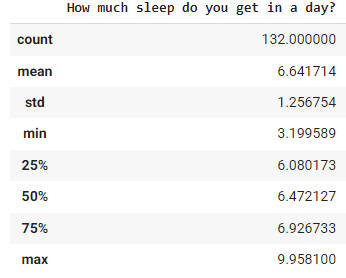
\includegraphics[width=8.5cm]{DF_SLP_Hours.png}
		\caption{Central Tendencies for Sleep Hours}
	\end{figure}
    
\end{frame}

\subsection{Verifying Central Limit Theorem for Sleep Hours}

\begin{frame}

	\frametitle{Sampling Distribution of Sleep Hours}
	
	\begin{figure}
		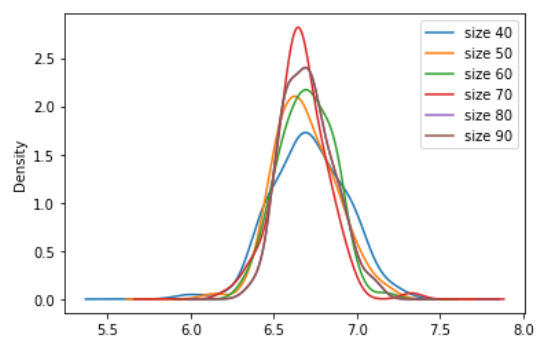
\includegraphics[width=8.5cm]{Normal_Dist.png}
		\caption{Sampling Distribution of Means of Sleep Hours}
	\end{figure}
	
	Sampling Distribution of Means tends to a normal distribution as the value of $n$ increases.
	
\end{frame}

\begin{frame}
    
    \frametitle{Sampling Mean Distribution}
    
    We also plotted the sampling mean distribution for sleep time by selecting random samples of varying sizes greater than 30. We can observe that as the random sample size increases the distribution is tending to be normal. From this we can observe that our data is not highly skewed and good representative of the population.

\end{frame}

\subsection{Hypothesis Testing for Sleep Hours}

\begin{frame}

    \frametitle{Hypothesis Testing}
    
    \begin{block}{Hypothesis}
        Students of IITH  sleep at least $6$ hrs on average. 
    \end{block}
    
\end{frame}

\begin{frame}
    
    \frametitle{Testing Hypothesis}
    
    \setcounter{equation}{0}
    
    \textbf{\underline{Calculation}}\\
    \\
    Null Hypothesis
    \begin{equation}
         (H_0) :  \mu - \mu_{0} \leq 0
    \end{equation}
    
    \bigskip
    
    Alternate Hypothesis
    \begin{equation}
        (H_a) : \mu - \mu_{0} > 0
    \end{equation}
    
    $\overline{X} = 6.641713$
    
    \bigskip
    
    $S = 1.256754$
    
    \bigskip 
    
    $ n = 132 , df = 131$
\end{frame}

\begin{frame}

    \frametitle{Testing Hypothesis}
    
    \textbf{Test Statistic}
    
    \bigskip
    
    $t = \cfrac{\overline{X} - \mu_0}{\cfrac{S}{\sqrt{n}}}  = \cfrac{6.641713 - 6}{\cfrac{1.256754}{\sqrt{132}}} = 5.844220$
    
    \bigskip
    
    $t_{\alpha, df} = t_{0.01, 131} = 2.355150$
    
    \bigskip
    
    Since $ t > t_{\alpha, df}$, we can reject $H_0$. 
    
    \begin{block}{Conclusion}
        So, we can conclude that students of IITH  sleep at least $6$ hrs on average.
    \end{block}
    
\end{frame}

\subsection{Data and Central Tendencies for Sleep Times}

\begin{frame}

    \frametitle{Central Tendencies for Sleep Times}
    
    \begin{figure}
		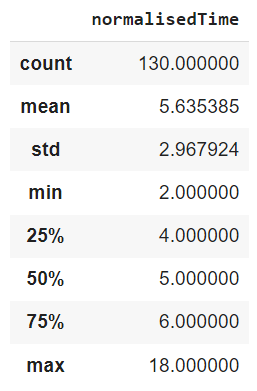
\includegraphics[width=4cm]{DF_Time_of_Sleep.png}
		\caption{Values of Central Tendencies (Time normalised about $8 PM$)}
	\end{figure}

\end{frame}

\begin{frame}

    The central tendencies are as follows : 
    
    \begin{block}
    
    Count : Refers to the number of students who have responded to this question
    
    \smallskip
    
    Mean : The mean time of sleep (Since it is normalized around 8 PM, the mean time of sleep would be $5.63 + 20 (8 PM) = 25.63$ (or) $1.63$, which is approximately $1:40$ AM).
    
    \smallskip
    
    Std : The standard deviation of sleep times 
    
    \smallskip
    
    Min : The earliest normalised sleep time (corresponds to $22:00$)
    
    \smallskip
    
    $25\%$ : The $1^{st}$ quartile
    
    \smallskip
    
    $50\%$ : The $2^{nd}$ quartile or median
    
    \smallskip
    
    $75\%$ : The $3^{rd}$ quartile 
    
    \smallskip
    
    Max : The last normalized sleep time (corresponds to $14:00$)
    
    \end{block}

\end{frame}

\subsection{Bar Graphs for Sleep Times}

\begin{frame}
    
    \frametitle{Sleep Time Analysis}

    \begin{figure}
    	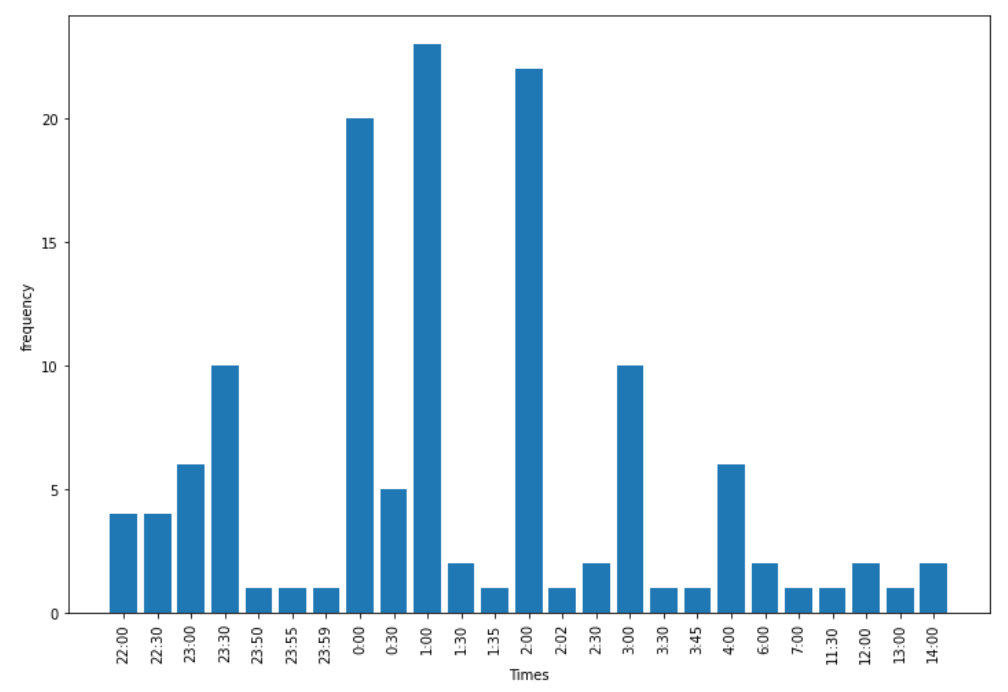
\includegraphics[width=8cm]{Sleep_Times.png}
    	\caption{The frequency of students sleeping at certain times}
    \end{figure}
    
    We can see that it is a \textbf{slightly right-skewed} and \textbf{unimodal}.

\end{frame}

\subsection{Verifying Central Limit Theorem for Sleep Times}

\begin{frame}

    \frametitle{Sampling Mean Distribution}
        
        \begin{figure}
		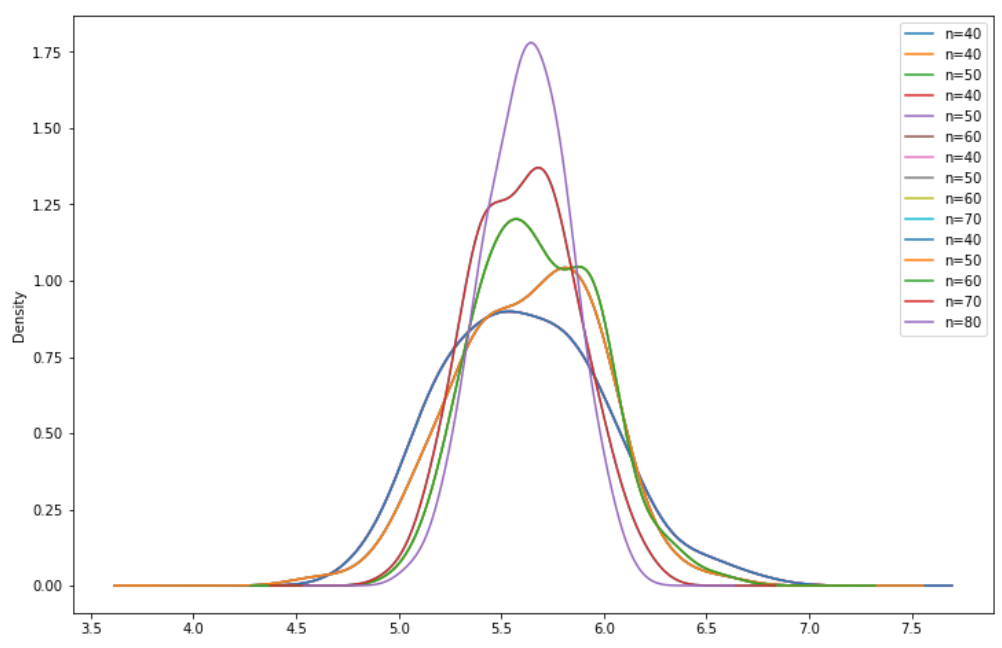
\includegraphics[width=8cm]{Sleep_Times_CLT.png}
		\caption{Data is consistent with Central Limit Theorem}
	\end{figure}
	
	Sampling Distribution of Means tends to a normal distribution as
    the value of n increases. 
    
\end{frame}

\section{Analysis of Study Times}

\subsection{Central Tendencies for Study Times}

\begin{frame}

    \frametitle{Central Tendencies for Study Times}
    
    \begin{figure}
		\includegraphics[width=4cm]{DF_Time_of_Study.png}
		\caption{Values of central Tendencies (Time normalised about $5 AM$)}
	\end{figure}
    
\end{frame}

\begin{frame}

    The central tendencies are as follows : 
    
    \begin{block}
    
    Count : Refers to the number of students who have responded to this question
    
    \smallskip
    
    Mean : The mean time of study (Since it is normalized around 5 AM, the mean time of sleep would be $11.15 + 5 = 16.15$, which is approximately $4:10 PM$).
    
    \smallskip
    
    Std : The standard deviation of study times 
    
    \smallskip
    
    Min : The earliest normalised study time (corresponds to $6:00 AM$)
    
    \smallskip
    
    $25\%$ : The $1^{st}$ quartile
    
    \smallskip
    
    $50\%$ : The $2^{nd}$ quartile or median
    
    \smallskip
    
    $75\%$ : The $3^{rd}$ quartile 
    
    \smallskip
    
    Max : The last normalized study time (corresponds to $2:00 AM$) 
    
    \end{block}

\end{frame}

\subsection{Bar Graphs for Study Times}

\begin{frame}

    \frametitle{Study Time Analysis}
    
	\begin{figure}
		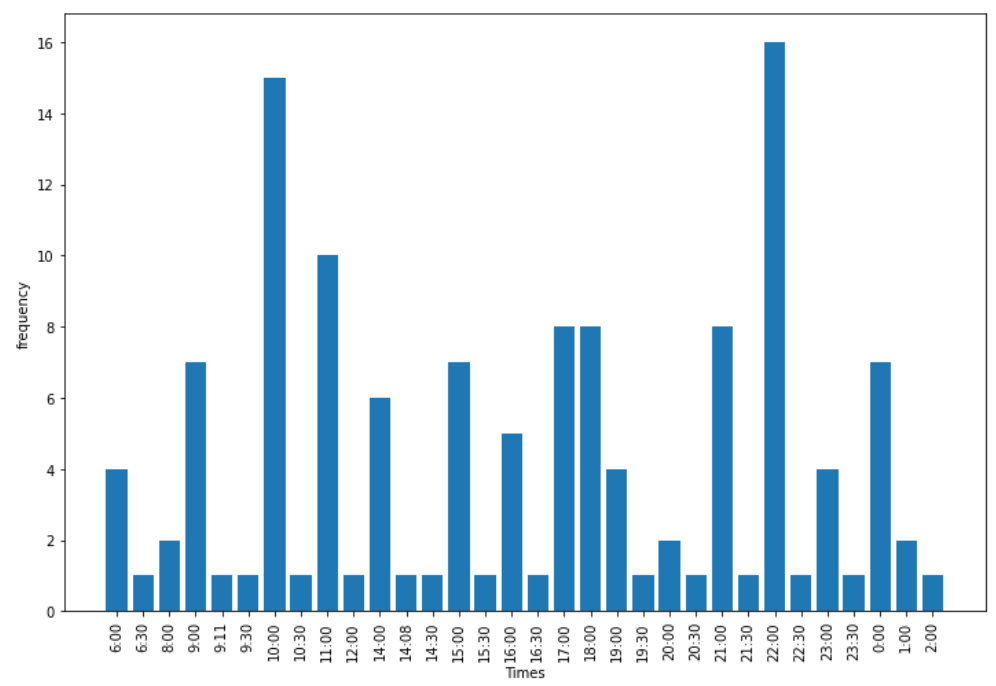
\includegraphics[width=10cm]{Bimodal.png}
		\caption{The frequency of students studying at certain times}
	\end{figure}
	
\end{frame}

\begin{frame}

    \frametitle{Study Time Analysis}
    
    From the plot, we can see that study times is near-symmetric, and a bimodal data set. 
    
    \bigskip
    
    One major reason for this occurrence is due to the fact that there are two groups of students, those who study early in the morning (before classes) and those who study at night (after classes). 
    
    \bigskip
    
    This leads to two peaks, which we can see at $10$ AM and $10$ PM. 
    
\end{frame}

\subsection{Verifying Central Limit Theorem for Study Times}

\begin{frame}

    \frametitle{Relation between Sleep Hours and Study Times}
    
    \begin{figure}
        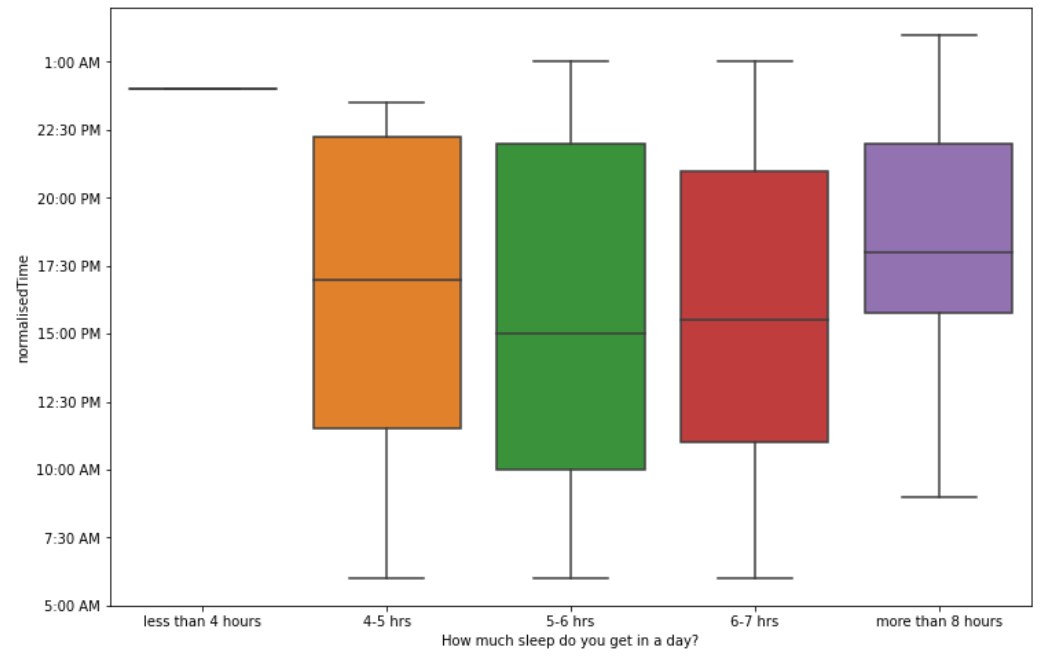
\includegraphics[width=10cm]{Box_Plt_Sleep_Hrs.png}
        \caption{Plot of Study Time and Hours of Sleep}
    \end{figure}
    
\end{frame}

\begin{frame}

    \frametitle{Inference from Box Plot}
    
    \textbf{Shape}: Slightly right-skewed, so most people tend to start studying early.
    
    \bigskip
    
    \textbf{Center}: People with moderate sleep tend to start studying earlier than people with extreme sleep habits.
    
    \bigskip
    
    \textbf{Spread}: The IQR of people who sleep more is less, so they consistently start studying in the evenings. 
    
\end{frame}

\begin{frame}

    \frametitle{Confidence Interval Estimation}

    We can say that with $95 \%$ confidence that the population mean time at which a person sleeps lies between ($1:07$ AM, $2:09$ AM).
    
    \bigskip
    
    We can say that with $95 \%$ confidence that the population mean time at which a person studies lies between ($15:12$ PM, $17:06$ PM).
    
\end{frame}

\section{Effects of Caffeine}

\begin{frame}

    \begin{block}{\textbf{Caffeine}}
    \end{block}
\end{frame}

% General Health Caffeine
\subsection{Information about Caffeine}

\begin{frame}
	\frametitle{General Information about Effects of Caffeine}
	
	Caffeine is one of the most consumed substances on a day-to-day basis. It is mainly consumed because of its profound effect on sleep and other cognitive functions. 
	
	\bigskip
	
	Known for its affect of sharpening the senses, it is majorly consumed by students to stay awake for longer periods of time, particularly for academic activities. 

	\bigskip 
	
	Studies have shown that caffeine dependence develops at relatively low daily doses and after short periods of regular daily use.
	
	\bigskip
	
	The risks to sleep and alertness of regular caffeine use are greatly underestimated by both the general population and physicians.
\end{frame}

% Start of data and analysis for caffeine
\subsection{Data and Central Tendencies}

\begin{frame}

    \setbeamerfont{caption}{size=\scriptsize}

    \frametitle{Relation between Caffeine intake and Sleep Times}
    
    \begin{columns}[c]
    
        \begin{column}{.5\textwidth}
        \begin{figure}
    		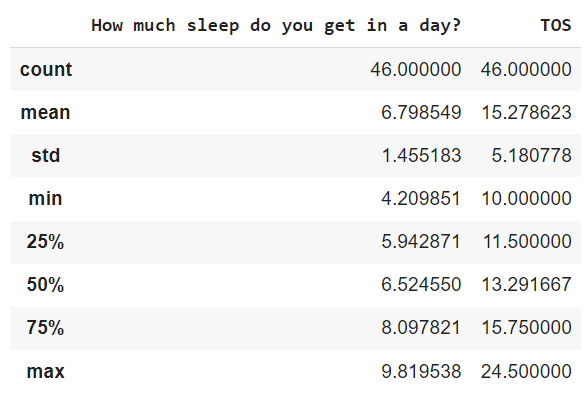
\includegraphics[width=4cm]{DF0.png}
    		\caption{\tiny{DF0 - No Caffeine intake}}
    	\end{figure}
    	\end{column}
    	
    	\begin{column}{.5\textwidth}
    	\begin{figure}
    		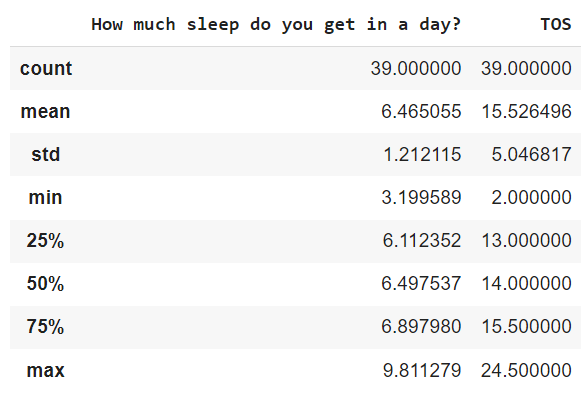
\includegraphics[width=4cm]{DF1.png}
    		\caption{\tiny{DF1 - One Caffeinated drink}}
    	\end{figure}
    	\end{column}
    	
    \end{columns}
    
    \begin{columns}[c]
    
        \begin{column}{.5\textwidth}
        \begin{figure}
    		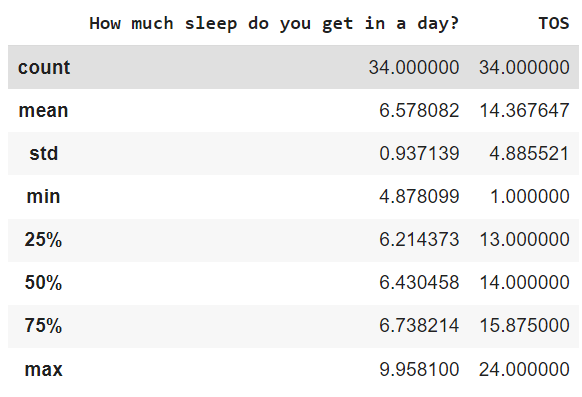
\includegraphics[width=4cm]{DF2.png}
    		\caption{\tiny{DF2 - Two Caffeine intake}}
    	\end{figure}
    	\end{column}
    	
    	\begin{column}{.5\textwidth}
    	\begin{figure}
    		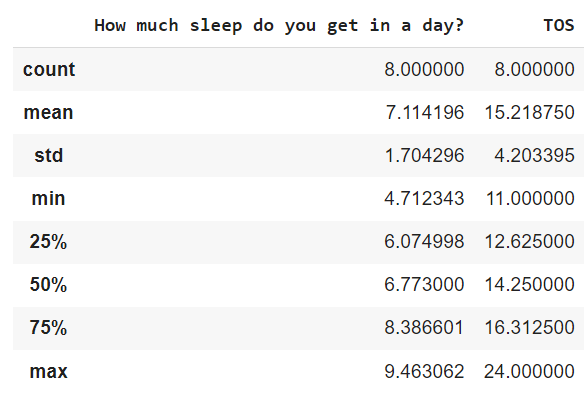
\includegraphics[width=4cm]{DF3.png}
    		\caption{\tiny{DF3 - More than Three Caffeinated drinks}}
    	\end{figure}
    	\end{column}
    	
    \end{columns}

\end{frame}

\begin{frame}
    The central tendencies are as follows : 
    
    \begin{block}
    
    Count : Size of the sample
    
    \smallskip
    
    Mean : Mean in the first column is mean of sleep hours in a day, and in the second column, it is mean time of sleep (normalized around $12$ PM). So, mean time of sleep is $12 + 15.27 = 27.27$ (or) $3.27$, which is around $3:20$ AM. 
    
    \smallskip
    
    Std : The standard deviation of study times 
    
    \smallskip
    
    Min : Column - 1 : The minimum number of sleep hours is $4.2$ hours. \\
          \hspace{9mm} Column - 2 : The earliest time of sleep is $10+ 12 = 22$ (or) $10$ PM. 
    
    \smallskip
    
    $25\%$ : The $1^{st}$ quartile
    
    \smallskip
    
    $50\%$ : The $2^{nd}$ quartile or median
    
    \smallskip
    
    $75\%$ : The $3^{rd}$ quartile 
    
    \smallskip
    
    Max : The last normalized study time (corresponds to $2:00$ AM) 
    
    \end{block}
\end{frame}

\subsection{Boxplots for the Categorical Variable}

\begin{frame}

    \frametitle{Relation between Caffeine intake and Sleep Hours}
    
    \textbf{Boxplots}
    
    \begin{figure}
		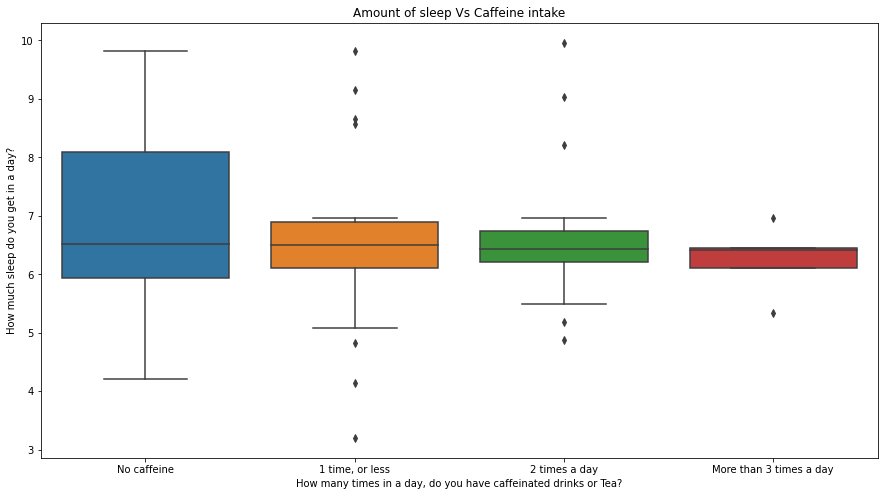
\includegraphics[width=10cm]{Caffeine_SleepHours.png}
		\caption{Caffeine effect on Sleep Hours}
	\end{figure}

\end{frame}

\begin{frame}

    \frametitle{Relation between Caffeine intake and Time of Sleep}
    
    \begin{figure}
		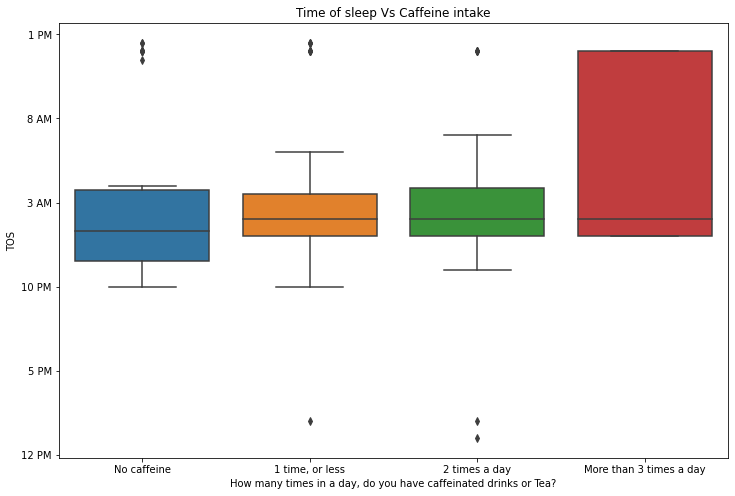
\includegraphics[width=10cm]{Caffeine_SleepTime.png}
		\caption{Caffeine effect on Time of Sleep}
	\end{figure}

\end{frame}

\subsection{Inferences}

\begin{frame}

	\frametitle{Inference from Box Plot - 1}
	
    \textbf{Shape}: For people who don't consume caffeine, the data is right- skewed so they tend to sleep less. But this value is greater than the number of sleep hours of other categories which consume caffeine. 
    
    \bigskip
    
    \textbf{Center}: All categories have nearly the same median.
    
    \bigskip
    
    \textbf{Spread}: We can observe that IQR decreases as caffeine consumption increases, so people who consume caffeine consistently sleep for the same amount of time.
    
    \bigskip
    
    \textbf{Outliers}: There are a considerable number of outliers among the moderate caffeine consuming categories.

\end{frame}

\begin{frame}

	\frametitle{Inference from Box Plot - 2}
	
	\textbf{Shape}: The box plot for high caffeine consumers is right skewed. More people in this category sleep early but this is late when compared with other categories.
	
	\bigskip
	
    \textbf{Center}: All categories have nearly the same mean.
    
    \bigskip
    
    \textbf{Spread}: We can observe that IQR of high caffeine consumers is more when compared with other categories, so they donot sleep consistently at the same time.
    
    \bigskip
    
    \textbf{Outliers}: There are a few outliers among less or no caffeine consuming categories.
    
\end{frame}

\begin{frame}

    \frametitle{Confidence Interval Calculation}
    
        \textbf{Confidence Interval for Number of Hours of Sleep}
        
        For a $95 \%$ confidence interval, the value of confidence coefficient is $\alpha = 0.05$. 
        
        \begin{equation}
            t_{\frac{\alpha}{2}} = 1.97823853 
        \end{equation}
        
        \begin{equation}
            \overline{X} - (t_{\frac{\alpha}{2}, df})(\cfrac{S}{\sqrt{n}}) \leq \mu \leq \overline{X} + (t_{\frac{\alpha}{2}, df})(\cfrac{S}{\sqrt{n}})
        \end{equation}
        
        \begin{equation}
            6.641 - (1.978)(\cfrac{1.251}{\sqrt{n}}) \leq \mu \leq 6.641 + (1,978)(\cfrac{1.251}{\sqrt{n}})
        \end{equation}
    
\end{frame}

\begin{frame}

	\frametitle{Confidence Interval Conclusions}

    \begin{enumerate}
        
        \item{We can say with \textit{95 \%} confidence that the number of hours of sleep is in the interval (6.42, 6.85)}
        
        \bigskip
        
        \item{We can say with \textit{95 \%} confidence that the number of hours of sleep of a person who \emph{\textbf{does not take}} any caffeine daily is in the interval (6.37, 7.22)}
        
        \bigskip
        
        \item{We can say with \textit{95 \%} confidence that the number of hours of sleep of a person who take \emph{\textbf{one}} caffeinated drink a day is in the interval (6.07, 6.85)}
        
    \end{enumerate}
    
\end{frame}

\begin{frame}

    \frametitle{Confidence Interval Conclusions}

    \begin{enumerate}\addtocounter{enumi}{3}
    
        \item{We can say with \textit{95 \%} confidence that the number of hours of sleep of a person who take \emph{\textbf{two}} caffeinated drinks a day is in the interval (6.25, 6.90)} 
        
        \bigskip
        
        \item{We can say with \texit{95 \%} confidence that the number of hours of sleep of a person who take \emph{\textbf{three}} caffeinated drinks a day is in the interval (5.78, 8.44)}
        
        \bigskip
        
        \item{We can say with \textit{95 \%} confidence that the number of hours of sleep of a person who take \emph{\textbf{greater than three}} caffeinated drinks a day is in the interval (5.58, 6.92)}
        
    \end{enumerate}

\end{frame}

\subsection{Hypothesis Testing and Calculation}

\begin{frame}
    
    \begin{block}{Hypothesis}
         Students who take caffeine sleep less than those who don't take caffeine. 
    \end{block}
    
\end{frame}


% \begin{frame}

%     \frametitle{Testing Hypothesis - 2}
    
%     \setcounter{equation}{0}
    
%     Null Hypothesis
%     \begin{equation}
%          (H_0) : S_{1}^{2} \leq S_{2}^{2}
%     \end{equation}
    
%     \bigskip
    
%     Alternate Hypothesis
%     \begin{equation}
%         (H_a) : S_{1}^{2} > S_{2}^{2}
%     \end{equation}
    
%     Test Statistic $(t) = \cfrac{S_{1}^{2}}{S_{2}^{2}} = 1.3353523$
    
%     \bigskip
    
%     $\alpha = 0.05, df_{1} = 45, df_{2} = 51$
    
%     \bigskip
    
%     $F_{\alpha, df_{1}, df_{2}} = 1.2806973$
    
%     \bigskip
    
%     Since $t \geq F_{\alpha, df_{1}, df_{2}}$, we can reject $H_0$. 
    
%     \bigskip
    
%     So, we can conclude that sleeping hours of those who take caffeine are more predictable (less variance) when compared with those who don't take caffeine. 
    
% \end{frame}

\begin{frame}

\frametitle{Testing Hypothesis}

\textbf{Calculation}\\
Null Hypothesis $(H_0) :  \mu_{c} - \mu_{nc} \geq 0$

\bigskip

Alternate Hypothesis $(H_a) : \mu_{c} - \mu_{nc} < 0$

\bigskip

$\overline{X}_{c} = 6.798548$

\bigskip

$n_{c} = 46$

\bigskip

$S_{c} = 1.455182$

\bigskip

$\overline{X}_{nc} = 6.544580$

\bigskip

$n_{nc} = 52$

\bigskip

$S_{nc} = 1.259272$

\end{frame}

\begin{frame}[fragile, t]

    \textbf{Test Statistic}
    
    \bigskip
    
    $ t = \cfrac{(\overline{X}_{c} - \overline{X}_{nc}) - (0)}{\sqrt{\cfrac{{(n_{c}-1)}S_{c}^{2}}{n_{c}+n_{nc} -2} + \cfrac{({n_{nc}}-1)S_{nc}^{2}}{n_{c}+n_{nc} -2}}(\sqrt{\cfrac{1}{n_{c}} + \cfrac{1}{n_{nc}}})} = 0.918048$
    
    \bigskip
    \bigskip
    $df = {n_{c}+n_{nc} -2} = 96$
    
\end{frame}

\begin{frame}[fragile, t]

    \textbf{Rejection Region Approach}
    
    \bigskip
    
    Reject $H_0$ if $t \leq -t_{\alpha, df}$ (let $\alpha$ = 0.05)
    
    \bigskip
    
    $t = 0.918048, t_{0.05, 96} = 1.6609612$ 
    
    \bigskip
    
    Hence, the hypothesis $H_{0}$ is not rejected. 
    
    \bigskip
    
    \begin{block}{Conclusion}
    The evidence is insufficient to conclude that those who take caffeine sleep less than those who don't take caffeine.
    \end{block}
    
\end{frame}

\section{Effects of Academics on Sleep}

\begin{frame}

    \begin{block}{\textbf{Academics}}
    \end{block}
\end{frame}

\subsection{Data and Central Tendencies}

\begin{frame}

    \frametitle{Central Tendencies for Lecture Watching Patterns}
    
    \begin{figure}
		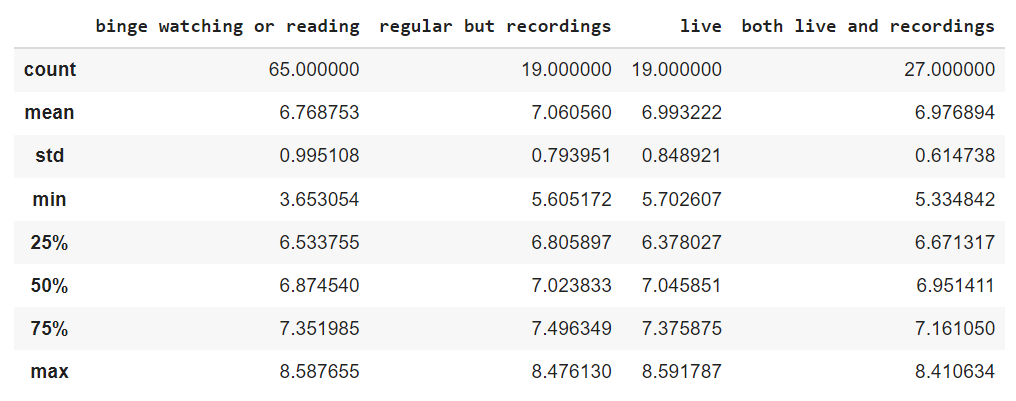
\includegraphics[width=11cm]{DF_Lectures.png}
		\caption{Lecture Watching Patterns}
	\end{figure}
    
\end{frame}

\begin{frame}

The central tendencies are as follows : 
    
    \begin{block}
    
    Count : Size of the sample (Here, number of students who binge watch lectures / who watch lectures live)
    
    \smallskip
    
    Mean : Mean in each column represents the mean of the hours of sleep the students of that category are getting. 
    
    \smallskip
    
    Std : The standard deviation of sleep times
    
    \smallskip
    
    Min : The least hours of sleep a student of that category is getting.
    
    \smallskip
    
    $25\%$ : The $1^{st}$ quartile
    
    \smallskip
    
    $50\%$ : The $2^{nd}$ quartile or median
    
    \smallskip
    
    $75\%$ : The $3^{rd}$ quartile 
    
    \smallskip
    
    Max : The maximum hours of sleep a student of that category is getting. 
    
    \end{block}
    
\end{frame}

\begin{frame}

    \frametitle{Central Tendencies for Assignment Submission Patterns}
    
    \begin{figure}
		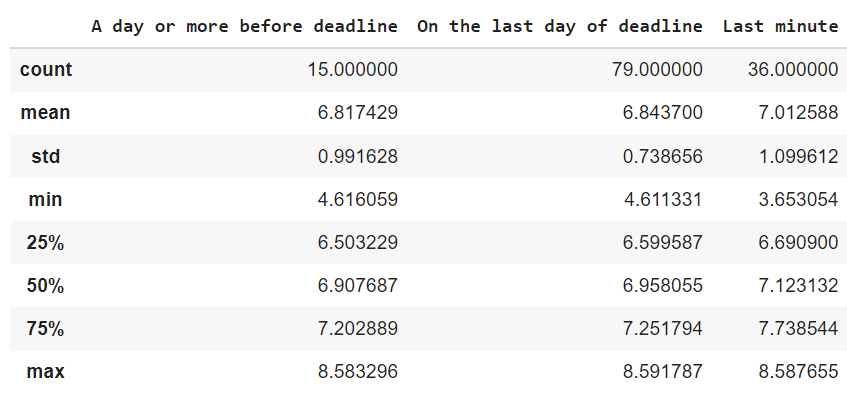
\includegraphics[width=11cm]{DF_Assignments.png}
		\caption{Assignment Submission Patterns}
	\end{figure}
    
\end{frame}

\subsection{Box Plots and Inferences}

\begin{frame}

    \frametitle{Box Plots}
    
    \begin{figure}
		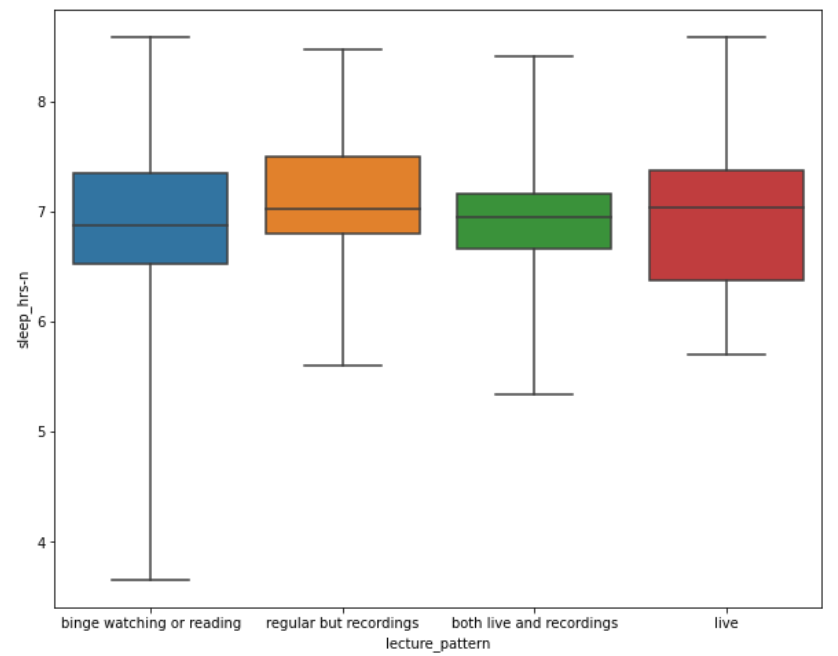
\includegraphics[width=8cm]{BoxPlt_Lecture.png}
		\caption{Box Plot for Modes of Lecture Watching}
	\end{figure}
	
\end{frame}

\begin{frame}

   \frametitle{Box Plots}
    
   \begin{figure}
		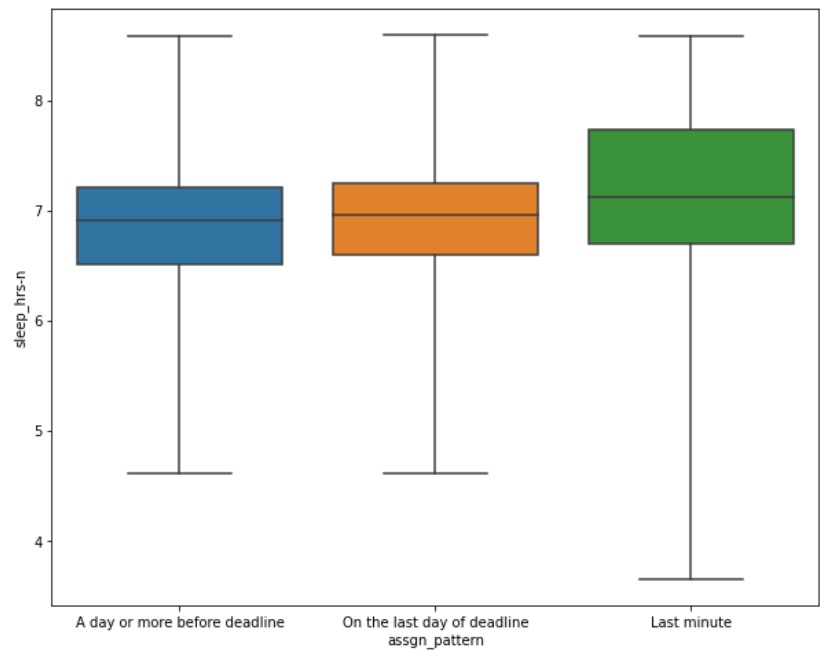
\includegraphics[width=8cm]{BoxPlt_Assignments.png}
		\caption{Box Plot for Assignment Submission Patterns}
	\end{figure}
    
\end{frame}


\begin{frame}

    \frametitle{Inference for Box Plot - 1}
    
    \textbf{Shape}: Category with left-skewness is people who watch live lectures and both live and recordings, so they tend to sleep for more time among themselves, which is different when compared with other categories. 
    
    \bigskip
    
    \textbf{Center}:  The average amount of sleep for the category of people watching recordings regularly is slightly higher than other categories.
    
    \bigskip
    
    \textbf{Spread}: The IQR of the category of people who watch both live lectures and recordings is the least, so they sleep more consistently when compared with other categories. Also, the range of sleep hours for the category of people who binge watch lectures is very high when compared with others, so the number of hours they sleep is very unpredictable.
    
\end{frame}

\begin{frame}

    \frametitle{Inference for Box Plot - 2}
    
    \textbf{Shape}: Only category with right-skewness is people who submit the assignment last minute, so they tend to sleep for less time among themselves. 
    
    \bigskip
    
    \textbf{Center}:  The average amount of sleep for the category of people is slightly increasing based on how close to the deadline they are submitting. 
    
    \bigskip
    
    \textbf{Spread}: The IQR of the category of people who submit the assignment last minute is highest, so they sleep less consistently when compared with other categories. 
    
\end{frame}

\subsection{Segmented Bar Charts and Inferences}

\begin{frame}

    \frametitle{Segmented Bar Chart}
    
   \begin{figure}
		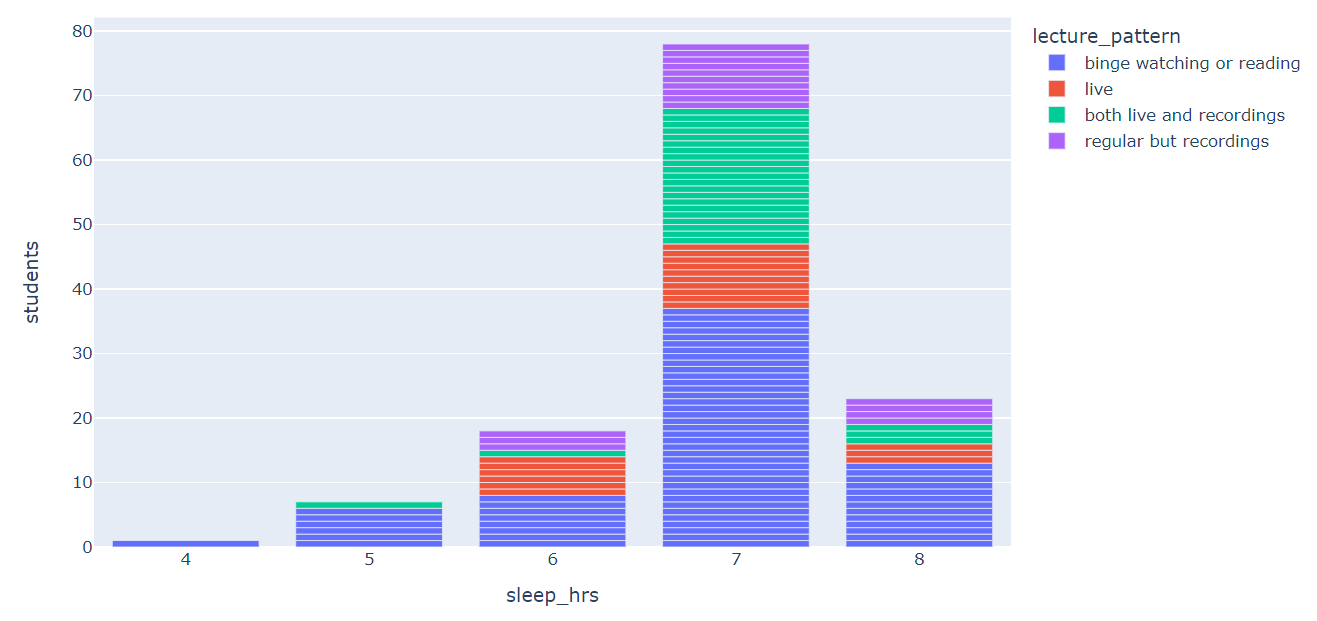
\includegraphics[width=12cm]{Seg_Barchart_Lecture_pattern.png}
		\caption{Segmented Bar Chart for Lecture Watching Patterns}
	\end{figure}
    
\end{frame}

\begin{frame}

    \frametitle{Segmented Bar Chart}
        
   \begin{figure}
		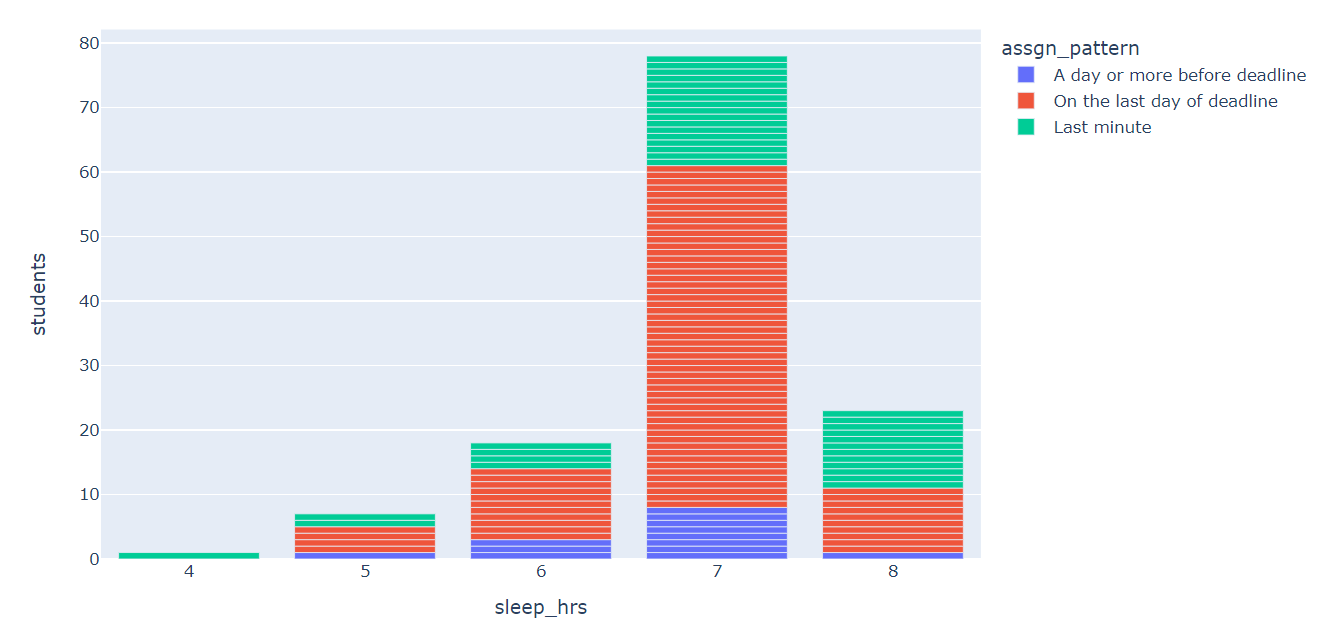
\includegraphics[width=12cm]{Seg_barchart_Assignments.png}
		\caption{Segmented Bar Chart for Assignment Submission Patterns}
	\end{figure}
    
\end{frame}

\begin{frame}
    
    \frametitle{Inferences from Segmented Bar Charts}
    
    \begin{block}{Inference from Segmented Bar Chart - 1}
        
        A higher proportion of students who watch lectures live, live and recordings sleep over 6 hours. 
        
    \end{block}
    
    \bigskip
    
    \begin{block}{Inference from Segmented Bar Chart - 2}
        
        For any quantity of sleep, there are more students who submit assignments on the last day than those who submit earlier.
        
    \end{block}
    
\end{frame}

\section{Sports and Social Activities}

\subsection{General Information about Sports and Social Activities}

\begin{frame}

    \begin{block}{\textbf{Sports and Social Activities}}
    
    \end{block}
    
\end{frame}

\begin{frame}

	\frametitle{Sports and Social Activities}
	
	Participating in sports activities can help people enhance their physical and mental health. 
	
	\bigskip
	
	For young students, participation in sports activities is crucial to avoid developing negative habits of spending leisure time. 
	
	\bigskip
	
	Common sports activities include playing football, basketball, badminton, cricket etc. and physical activities commonly include yoga, cycling, jogging etc. 
	
	\bigskip
    
	Studies in Foreign Colleges show that 29 out of the 34 conducted studies concluded that exercise improved sleep duration. 
	
\end{frame}

\subsection{Data and Central Tendencies}

\begin{frame}

    \setbeamerfont{caption}{size=\scriptsize}
    
	\frametitle{Central Tendencies for Recreational Activities}
	
	\begin{columns}[c]
	
	\begin{column}{.5\textwidth}
    	\begin{figure}
    		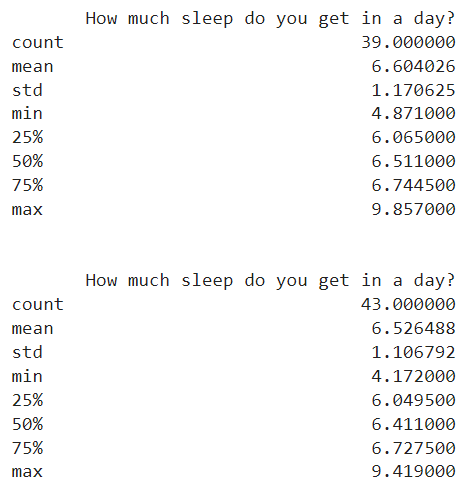
\includegraphics[width=6cm]{DF_List_1.png}
    		\caption{
    		\tiny{Effect of 1-2 hours, 2-3 hours of Recreational activities on Sleep Hours}
    		}
    	\end{figure}
	\end{column}

    \begin{column}{.5\textwidth}
    	\begin{figure}
    		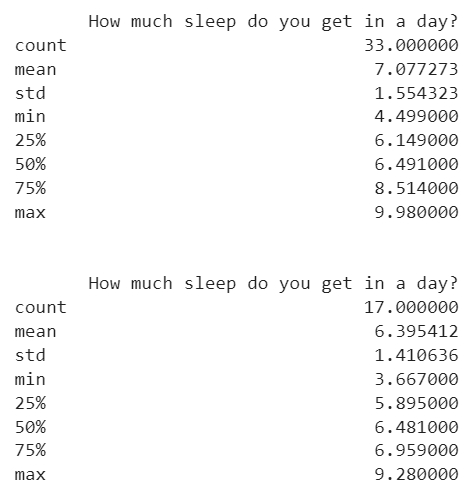
\includegraphics[width=6cm]{DF_List_2.png}
    		\caption{
    		\tiny{Effect of 4-5 hours, 6 or more hours of Recreational activities on Sleep Hours}
    		}
    	\end{figure}
	\end{column}
	
    \end{columns}	
	
\end{frame}

\begin{frame}

    \setbeamerfont{caption}{size=\scriptsize}
    
	\frametitle{Central Tendencies for Sports and Social Activities}
	
	\begin{columns}[c]
	
	\begin{column}{.5\textwidth}
    	\begin{figure}
    		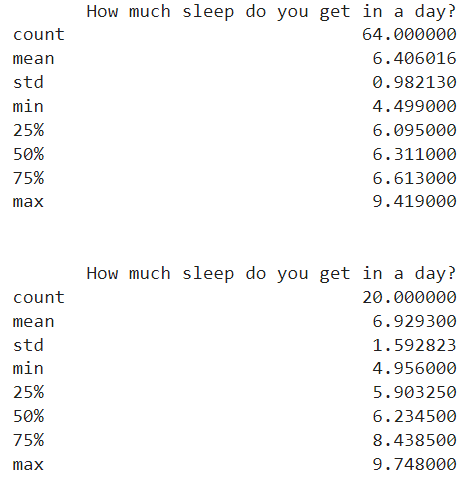
\includegraphics[width=6cm]{DF_List_3.png}
    		\caption{
    		\tiny{Effect of 1-2 hours, 2-3 hours of Sports and Gym activities on Sleep Hours} 
    		}
    	\end{figure}
	\end{column}

    \begin{column}{.5\textwidth}
    	\begin{figure}
    		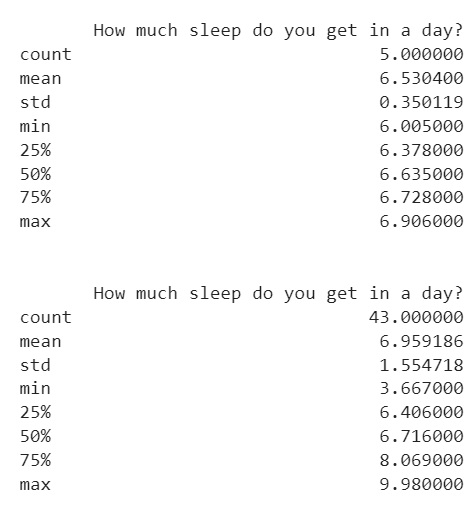
\includegraphics[width=6cm]{DF_List_4.png}
    		\caption{
    	    \tiny{Effect of 4 or more hours, and no Sports and Gym activities on Sleep Hours}
    		}
    	\end{figure}
	\end{column}
	
    \end{columns}
	
\end{frame}

\subsection{Box Plots}

\begin{frame}
	\frametitle{Box Plot for Recreational Activities}
	
    \begin{figure}
		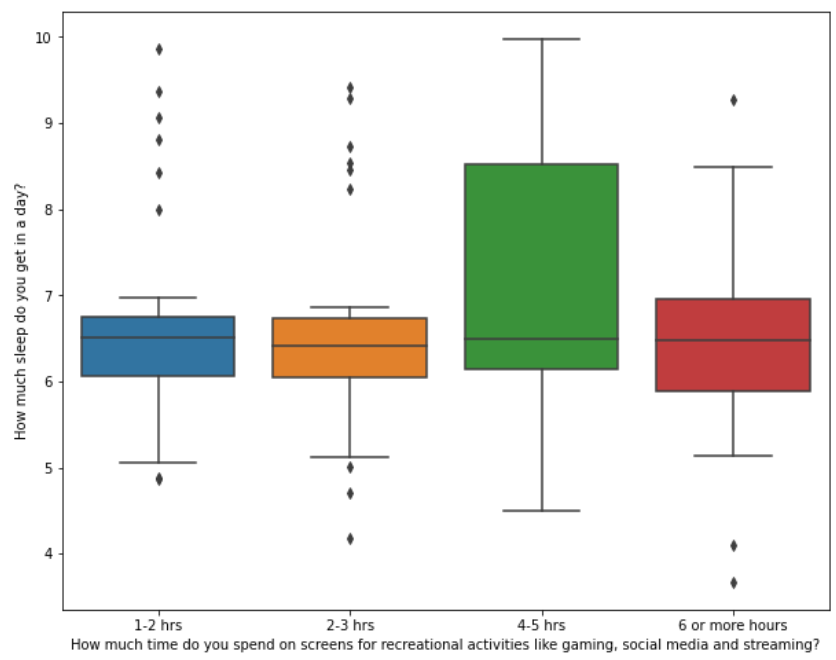
\includegraphics[width=8.5cm]{BoxPlt_Recreational.png}
		\caption{Effect of Recreational activities on Sleep Hours}
	\end{figure}
	
\end{frame}

\begin{frame}
	\frametitle{Box Plot for Sports and Social Activities}
	
	\begin{figure}
		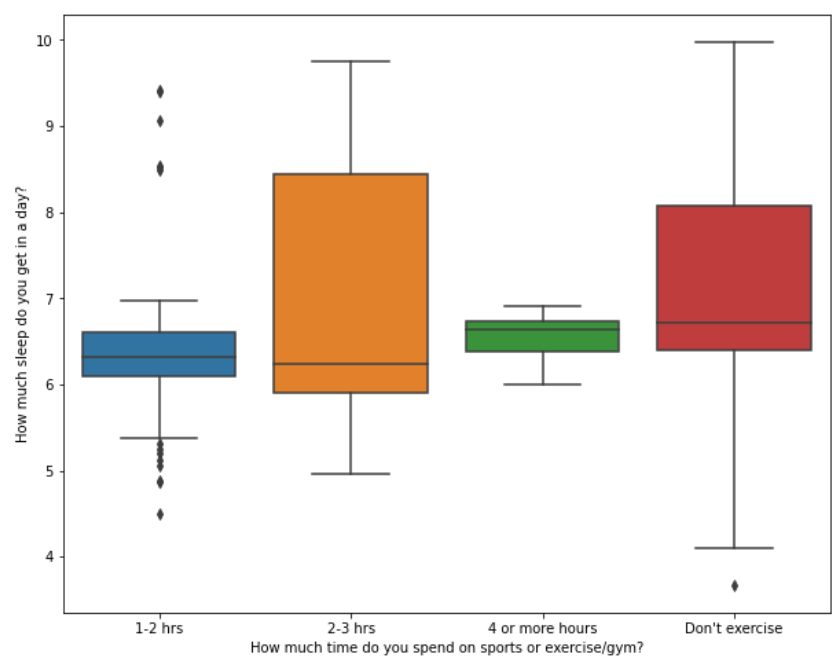
\includegraphics[width=8.5cm]{BoxPlt_Sports.png}
		\caption{Effect of Sport activities on Sleep Hours}
	\end{figure}

\end{frame}

\subsection{Inferences from Box Plots}

\begin{frame}

    \frametitle{Inference from Box Plot - 1}
    
    \textbf{Shape}: Only category with right skewness is people who spend $4-5$ hours on recreation, so they tend to sleep for less time among themselves. 
    
    \bigskip
    
    \textbf{Center}:  The median of all the categories are nearly the same.
    
    \bigskip
    
    \textbf{Spread}: The IQR of the category of people who spend $4-5$ hours on recreation is highest, so they sleep less consistently when compared with other categories.
    
\end{frame}

\begin{frame}
    
    \frametitle{Inference from Box Plot - 2}
    
    \textbf{ Shape}: Only category with left skewness is people who spend $4$ or more hours on sports activities, so they tend to sleep for less time among themselves and exactly the opposite applies for the remaining categories.
    
    \bigskip
    
    \textbf{ Center}:  The median of people who do not exercise is slightly higher than other categories. The people who do not play sports tend to sleep more than others. 
    
    \bigskip
    
    \textbf{Spread}: The IQR of the category of people who spend $4-5$ hours on recreation is least, so they sleep more consistently when compared with other categories. 
    
\end{frame}

\subsection{Confidence Interval Estimation}

\begin{frame}
	\frametitle{Confidence Interval Estimation}
	
	\begin{enumerate}
	\item{We can say with \textit{95 \%} confidence that the number of hours of sleep is in the interval who spends 1-2 hrs on recreational activities (6.10, 6.96)}
	
	\bigskip
	
    \item{We can say with \textit{95 \%} confidence that the number of hours of sleep is in the interval who spends 2-3 hrs on recreational activities (6.15, 6.84)}
    
    \bigskip
    
    \item{We can say with \textit{95 \%} confidence that the number of hours of sleep is in the interval who spends 4-5 hrs on recreational activities (6.56, 7.72)}
    
    \bigskip
    
    \item{We can say with \textit{95 \%} confidence that the number of hours of sleep is in the interval who spends 6 or more hours on recreational activities (5.66, 7.30)}
	\end{enumerate}
	
\end{frame}

\begin{frame}
	\frametitle{Confidence Interval Estimation}
	
    \begin{enumerate}\addtocounter{enumi}{4}
    
    \item{We can say with \textit{95 \%} confidence that the number of hours of sleep is in the interval who spends 1-2 hrs on sports/gym (6.09, 6.65)}
    
    \bigskip
    
    \item{We can say with \textit{95 \%} confidence that the number of hours of sleep is in the interval who spends 2-3 hrs on sports/gym (6.17, 7.80)}
    
    \bigskip
    
    \item{We can say with \textit{95 \%} confidence that the number of hours of sleep is in the interval who spends 4 or more hours on sports/gym (6.13, 6.75)}
    
    \bigskip
    
    \item{We can say with \textit{95 \%} confidence that the number of hours of sleep is in the interval who spends Don't exercise on sports/gym (6.48, 7.47)}
    
    \end{enumerate}
    
\end{frame}

%%%%%%%%%%%%%%%%%
% PUSH TO TOP 

%%%%%%%%%%%%%%%%%

\section{Hypothesis Testing}

\subsection{Recreational Hypothesis}

\begin{frame}

    \frametitle{Hypothesis Testing}
    
    \begin{block}{Hypothesis}
    A student that spends 1-3 hours on recreational activities a day on average sleeps less than a student that spends more than 4 hours on the same activities a day. 
    \end{block}

    \textbf{\underline{Calculation}}\\
    \\
    Null Hypothesis
    \begin{equation}
         (H_0) :  \mu_{1-3} - \mu_{>4} \geq 0
    \end{equation}
    
    \bigskip
    
    Alternate Hypothesis
    \begin{equation}
        (H_a) : \mu_{1-3} - \mu_{>4} < 0
    \end{equation}

\end{frame}

\begin{frame}

$\overline{X}_{1-3} = 6.565374$

\bigskip

$n_{1-3} = 39 + 43 = 82$

\bigskip

$S_{1-3} = \sqrt{\cfrac{1.170625^2}{n_{1-2}}+ \cfrac{1.106792^2}{n_{2-3}}} = 0.212241$

\bigskip

$\overline{X}_{>4} = 6.7363425$

\bigskip

$n_{>4} = 33 + 17 = 50$

\bigskip

$S_{>4} = \sqrt{\cfrac{1.554323^2}{n_{4-5}}+ \cfrac{1.410636^2}{n_{>6}}} = 0.4361906$

\end{frame}

\begin{frame}

    \textbf{Test Statistic}
    
    \bigskip
    
    $ t = \cfrac{(\overline{X}_{1-3} - \overline{X}_{>4}) - (0)}{\sqrt{\cfrac{S_{1-3}^{2}}{n_{1-3}} + \cfrac{S_{>4}^{2}}{n_{>4}}}} = \cfrac{6.565374 - 6.7363425}{\sqrt{0.0045811}} = -2.525969$
    
    \bigskip
    
    $ c= \cfrac{\cfrac{S_{1-3}^{2}}{n_{1-3}}}{\cfrac{S_{1-3}^{2}}{n_{1-3}} + \cfrac{S_{>4}^{2}}{n_{>4}}} = 0.16937213$
    
    \bigskip
    
    $ df = \cfrac{(n_{1-3} - 1)(n_{>4} - 1)}{(1 - c)^{2}(n_{1-3}- 1) + (c^2)(n_{>4} - 1)} = 69.27787972 \sim 69$
    
\end{frame}

\begin{frame}

    \textbf{Rejection Region Approach}
    
    Reject $H_0$ if $t \leq -t_{\alpha, df}$ (let $\alpha$ = 0.05)
    
    \bigskip
    
    $t = -2.525969, t_{0.05, 69} = 1.6673$ 
    
    \bigskip
    
    Hence, the hypothesis $H_{0}$ is rejected. 
    
    \bigskip
    
    \begin{block}{Conclusion}
    We can conclude that a student that spends 1-3 hours on recreational activities a day on average sleeps less than a student that spends more than 4 hours on the same activities a day. 
    \end{block}
    
\end{frame}

%%%%%%%%%%%%%%%%%%%%%

\subsection{Sports Hypothesis}

\begin{frame}
\frametitle{Hypothesis Testing}

\begin{block}{Hypothesis}

A student who does not exercise sleeps more on average than a student who exercises. 

\end{block}

    \textbf{\underline{Calculation}}\\
    \\
    Null Hypothesis
    \begin{equation}
         (H_0) :  \mu_{e} - \mu_{de} \geq 0
    \end{equation}
    
    \bigskip
    
    Alternate Hypothesis
    \begin{equation}
        (H_a) : \mu_{e} - \mu_{de} < 0
    \end{equation}

\end{frame}

\begin{frame}

$\overline{X}_{e} = 6.6219053$

\bigskip

$n_{e} = 64 + 20 + 5 = 89$

\bigskip

$S_{e} = \sqrt{\cfrac{0.982130^2}{n_{1-2}}+ \cfrac{1.592823^2}{n_{2-3}} + \cfrac{0.350119^2}{n_{>4}}} = 0.40797361$

\bigskip

$\overline{X}_{d} = 6.959186$

\bigskip

$n_{d} = 43$

\bigskip

$S_{d} = 1.554718$

\end{frame}

\begin{frame}

    \textbf{Test Statistic}
    
    \bigskip
    
    $ t = \cfrac{(\overline{X}_{e} - \overline{X}_{de}) - (0)}{\sqrt{\cfrac{S_{e}^{2}}{n_{e}} + \cfrac{S_{de}^{2}}{n_{de}}}} = \cfrac{6.621905333 - 6.959186}{\sqrt{0.0580829}} = -1.399482137$
    
    \bigskip
    
    $ c= \cfrac{\cfrac{S_{e}^{2}}{n_{e}}}{\cfrac{S_{e}^{2}}{n_{e}} + \cfrac{S_{de}^{2}}{n_{de}}} = 0.032197782$
    
    \bigskip
    
    $df = \cfrac{(n_{e} - 1)(n_{de} - 1)}{(1 - c)^{2}(n_{e}- 1) + (c^2)(n_{de} - 1)} \sim 45$
    
\end{frame}

\begin{frame}

    \textbf{Rejection Region Approach}
    
    Reject $H_0$ if $t \leq -t_{\alpha, df}$ (let $\alpha$ = 0.05)
    
    \bigskip
    
    $t = -1.399482137, t_{0.05, 42} = 1.682$ 
    
    \bigskip
    
    Hence, the hypothesis $H_{0}$ is not rejected. 
    
    \bigskip
    
    \begin{block}{Conclusion}
    Insufficient evidence to conclude that a student who does not exercise sleeps more on average than a student who exercises. 
    \end{block}
    
\end{frame}

\begin{frame}

    \frametitle{Contributions of each team member}
    
    Prajwaldeep Kamble - Effect of Academics on Response Variables + Google Forms Design
    
    \bigskip
    
    Anurag Gopi - Effect of Academics on Response Variables
    
    \bigskip
    
    Krishna Teja Chilukuri - Effect of Caffeine on Response Variables + Hypothesis Testing of Caffeine
    
    \bigskip
    
    Venkata Raghav Ambati - Effect of Caffeine on Response Variables + Google Forms Distribution
 
\end{frame}
 
\begin{frame}

    \frametitle{Contributions of each team member}
    
    Nikhil Kongara - Study of Response Variables 
    
    \bigskip
    
    Karthik Kurugodu - Effect of Sports and Recreational Activities on Response Variables + Hypothesis Testing of Recreational Activities
    
    \bigskip
    
    VKS Deepak Reddy - Effect of Sports and Recreational Activities on Response Variables + Topic of Study 
    
    \bigskip
    
    Tata Sai Manoj - Latex Report + Hypothesis Testing of Sport Activities + Image Handling
    
    \bigskip
    
    Sumanth NR - Latex Report + Refining Data + Study Time Analysis

\end{frame}

\section{References}

\begin{frame}

	\frametitle{References}
	
	\begin{enumerate}
	    \item{https://www.ncbi.nlm.nih.gov/pmc/articles/PMC5385214/}
	    \item{\href{https://www.researchgate.net/publication/261159147_Impacts_of_sports_on_students'_life}{Research Gate article}}
	\end{enumerate}
	
\end{frame}

\end{document}